\documentclass[12pt,a4paper]{report}

% ==============================================================================
% PACKAGES
% ==============================================================================
\usepackage[top=2.2cm, bottom=2.4cm, left=2.8cm, right=2.3cm]{geometry}
\usepackage{times}
\usepackage{setspace}
\usepackage{xcolor}
\usepackage{graphicx}
\usepackage{grffile}
\usepackage{array}
\usepackage{longtable}
\usepackage{booktabs}
\usepackage{tabularx}
\usepackage{colortbl}
\usepackage{titlesec}
\usepackage{fancyhdr}
\usepackage[normalem]{ulem}
\usepackage{parskip}
\usepackage{enumitem}
\usepackage{listings}
\usepackage{microtype}
\usepackage{caption}
\usepackage{float}
\usepackage{amsmath}
\usepackage{amssymb}
\usepackage{needspace}
\usepackage{tikz}
\usetikzlibrary{shapes.geometric, arrows.meta, positioning, fit, calc, backgrounds}
\usepackage{xurl}
\usepackage{hyphenat}
\usepackage{hyperref}

\graphicspath{{./}{screenshots/}}

% ==============================================================================
% EXACT COLOR DEFINITIONS
% ==============================================================================
\definecolor{pdfred}{RGB}{204, 0, 0}
\definecolor{pdfnavy}{RGB}{0, 32, 96}
\definecolor{pdfgreen}{RGB}{46, 125, 50}
\definecolor{pdffootrule}{RGB}{140, 50, 20}
\definecolor{codebg}{RGB}{247, 248, 250}
\definecolor{amber}{RGB}{217, 119, 6}
\definecolor{slate}{RGB}{71, 85, 105}

% ==============================================================================
% PAGE LAYOUT & TYPOGRAPHY
% ==============================================================================
\onehalfspacing
\setlength{\parindent}{0pt}
\setlength{\parskip}{5pt}
\emergencystretch=3em
\hfuzz=1pt
\widowpenalty=10000
\clubpenalty=10000

% TikZ Page Frame Command (10mm inset on all sides)
\newcommand{\drawpageframe}{%
  \begin{tikzpicture}[remember picture,overlay]
    \draw[line width=1.2pt, color=black] 
      ($(current page.north west) + (10mm,-10mm)$) 
      rectangle 
      ($(current page.south east) + (-10mm,10mm)$);
  \end{tikzpicture}%
}

% Header & Footer Settings
\pagestyle{fancy}
\fancyhf{}
\renewcommand{\headrulewidth}{0pt}
\renewcommand{\footrulewidth}{1.8pt}
\renewcommand{\footrule}{\hbox to\headwidth{\color{pdffootrule}\leaders\hrule height \footrulewidth\hfill}}
\fancyfoot[R]{\thepage}

% Chapter & Section Heading Formatting
\titleformat{\chapter}[display]
  {\normalfont\bfseries\centering}
  {\MakeUppercase{\chaptertitlename\ --\ \thechapter}}
  {1ex}
  {\MakeUppercase}
\titlespacing*{\chapter}{0pt}{-10pt}{20pt}

\titleformat{\section}
  {\normalfont\normalsize\bfseries}
  {\thesection}{1em}{}
\titlespacing*{\section}{0pt}{12pt}{6pt}

\titleformat{\subsection}
  {\normalfont\normalsize\bfseries}
  {\thesubsection}{1em}{}
\titlespacing*{\subsection}{0pt}{8pt}{4pt}

% Listings Configuration
\lstset{
  backgroundcolor=\color{codebg},
  basicstyle=\ttfamily\footnotesize,
  breaklines=true,
  frame=single,
  rulecolor=\color{slate!30},
  keywordstyle=\color{pdfnavy}\bfseries,
  commentstyle=\color{pdfgreen}\itshape,
  stringstyle=\color{pdfred},
  numbers=none,
  tabsize=2,
  showstringspaces=false,
  captionpos=b
}

% Hyperref Configuration
\hypersetup{
  colorlinks=true,
  linkcolor=pdfnavy,
  citecolor=pdfnavy,
  urlcolor=pdfnavy,
  pdfborder={0 0 0}
}

\begin{document}

% ==============================================================================
% PAGE 1 — COVER / TITLE PAGE
% ==============================================================================
\begin{titlepage}
\drawpageframe
\thispagestyle{empty}
\centering

\vspace*{0.2cm}

{\fontsize{18pt}{22pt}\selectfont \textbf{\textcolor{pdfnavy}{SMART CPU SCHEDULER WITH DYNAMIC PRIORITY ADJUSTMENT}}\par}

\vspace{0.6cm}

{\fontsize{12pt}{15pt}\selectfont \textbf{A PROJECT REPORT}\par}

\vspace{0.3cm}

{\fontsize{11pt}{14pt}\selectfont \textit{Submitted in partial fulfillment of the requirements for the award of the degree of}\par}

\vspace{0.4cm}

{\fontsize{13pt}{16pt}\selectfont \textbf{\textcolor{pdfred}{BACHELOR OF TECHNOLOGY}}\par}

\vspace{0.2cm}

{\fontsize{11pt}{14pt}\selectfont \textit{in}\par}

\vspace{0.2cm}

{\fontsize{12pt}{15pt}\selectfont \textbf{\textcolor{pdfnavy}{DEPARTMENT OF COMPUTER SCIENCE AND ENGINEERING}}\par}

\vspace{0.4cm}

{\fontsize{11pt}{14pt}\selectfont \textit{by}\par}

\vspace{0.3cm}

{\color{pdfred}\bfseries
\begin{tabular}{ll}
BHARGAVA & 2520090169 \\
HANISH   & 2520090107 \\
TEJA     & 2520090162 \\
PARDHU   & 2520090043 \\
\end{tabular}
\par}

\vspace{0.4cm}

{\fontsize{11pt}{14pt}\selectfont \textit{Under the esteemed guidance of}\par}
\vspace{0.2cm}
{\fontsize{12pt}{14pt}\selectfont \textbf{\textcolor{pdfred}{Mrs. Alekhya}}\par}
{\fontsize{10.5pt}{13pt}\selectfont Assistant Professor\par}

\vspace{0.4cm}

\IfFileExists{kl_logo.png}{%
  \includegraphics[width=3.2cm,keepaspectratio]{kl_logo.png}\par
}{%
  \vspace{2.2cm}%
}

\vspace{0.4cm}

{\fontsize{12pt}{15pt}\selectfont \textbf{\textcolor{pdfred}{Koneru Lakshmaiah Education Foundation}}\par}
{\fontsize{10.5pt}{13pt}\selectfont (KL Deemed to be University)\par}
{\fontsize{9.5pt}{12pt}\selectfont Off-Campus: Bachupally-Gandimaisamma Road, Bowrampet, Hyderabad, Telangana -- 500 043.\par}
{\fontsize{9.5pt}{12pt}\selectfont Phone: 7815926816 \quad | \quad Website: \url{www.klh.edu.in}\par}
{\fontsize{10.5pt}{13pt}\selectfont \textbf{Academic Year: 2026--2027}\par}

\end{titlepage}

% ==============================================================================
% PAGE 2 — DECLARATION
% ==============================================================================
\newpage
\drawpageframe
\thispagestyle{empty}

\begin{center}
{\fontsize{16pt}{20pt}\selectfont \textbf{DECLARATION}\par}
\end{center}

\vspace{1.2cm}

The Project Report entitled \textbf{``Smart CPU Scheduler with Dynamic Priority Adjustment''} is a record of Bonafide work of \textcolor{pdfgreen}{\textbf{BHARGAVA -- 2520090169, HANISH -- 2520090107, TEJA -- 2520090162, PARDHU -- 2520090043}} submitted in partial fulfillment for the award of B. Tech in Computer Science and Engineering to the K L University. The results embodied in this report have not been copied from any other departments/University/Institute.

\vspace{4.5cm}

\begin{flushright}
\begin{tabular}{ll}
\textbf{Signature of the Student(s):} & \\[1.0cm]
BHARGAVA & (2520090169) \dotfill \\[0.4cm]
HANISH   & (2520090107) \dotfill \\[0.4cm]
TEJA     & (2520090162) \dotfill \\[0.4cm]
PARDHU   & (2520090043) \dotfill \\
\end{tabular}
\end{flushright}

\vfill
\begin{flushleft}
Date: \today \\
Place: Hyderabad
\end{flushleft}

% ==============================================================================
% PAGE 3 — CERTIFICATE
% ==============================================================================
\newpage
\drawpageframe
\thispagestyle{empty}

\begin{center}
{\fontsize{16pt}{20pt}\selectfont \textbf{CERTIFICATE}\par}
\end{center}

\vspace{1.0cm}

This is to certify that the mini project based report entitled \textbf{``Smart CPU Scheduler with Dynamic Priority Adjustment''} is a bonafide work done and submitted by \textcolor{pdfgreen}{\textbf{BHARGAVA -- 2520090169, HANISH -- 2520090107, TEJA -- 2520090162, PARDHU -- 2520090043}}, in partial fulfillment of the requirements for the award of the degree of \textcolor{pdfred}{\textbf{BACHELOR OF TECHNOLOGY}} in Department of Computer Science Engineering, K L (Deemed to be University), during the academic year \textcolor{pdfred}{\textbf{2026--2027}}.

\vspace{2.5cm}

\begin{flushright}
\textbf{Mrs. Alekhya} \\
Assistant Professor \\
Project Guide
\end{flushright}

\vspace{2.5cm}

\noindent
\begin{tabularx}{\textwidth}{@{}X r@{}}
\textbf{Course Coordinator} & \textbf{Head of the Department} \\
Department of CSE & Department of CSE \\
KL University, Hyderabad & KL University, Hyderabad \\
\end{tabularx}

% ==============================================================================
% PAGE 4 — ACKNOWLEDGEMENT
% ==============================================================================
\newpage
\pagenumbering{roman}
\setcounter{page}{1}
\drawpageframe
\thispagestyle{empty}
\phantomsection\label{ack}

\begin{center}
{\fontsize{16pt}{20pt}\selectfont \textbf{ACKNOWLEDGEMENT}\par}
\end{center}

\vspace{0.8cm}

The success in this project would not have been possible but for the timely help and guidance rendered by many people. We wish to express our sincere thanks to all those who assisted us in one way or the other for the completion of our project.

Our greatest appreciation to our Guide \textcolor{pdfred}{\textbf{Mrs. Alekhya}}, Assistant Professor, Department of Computer Science and Engineering, whose support and guidance cannot be expressed in words.

We express our gratitude to the Head of the Department of Computer Science Engineering for providing us with adequate facilities and means to complete this project-based Lab.

We thank all teaching and non-teaching staff who assisted us directly or indirectly. Finally, we sincerely thank our parents, friends and classmates for their kind help and cooperation.

\vspace{3.5cm}

\begin{flushright}
\textbf{Team Members:} \\[0.4cm]
BHARGAVA \quad (2520090169) \\[0.2cm]
HANISH   \quad (2520090107) \\[0.2cm]
TEJA     \quad (2520090162) \\[0.2cm]
PARDHU   \quad (2520090043) \\
\end{flushright}

% ==============================================================================
% PAGE 5 — ABSTRACT
% ==============================================================================
\newpage
\thispagestyle{plain}
\phantomsection\label{abstract}

\begin{center}
{\fontsize{16pt}{20pt}\selectfont \textbf{ABSTRACT}\par}
\end{center}

\vspace{0.8cm}

Modern operating systems face a critical challenge: scheduling CPU resources fairly across multiple concurrent processes while preventing process starvation. Traditional scheduling algorithms such as First-Come-First-Served (FCFS), Round Robin, and static Priority Scheduling suffer from inherent limitations --- FCFS ignores urgency, Round Robin treats all processes identically regardless of priority, and static Priority Scheduling causes indefinite starvation of low-priority processes.

This project designs and implements a Smart CPU Scheduler with Dynamic Priority Adjustment using an aging-based algorithm in C. The core scheduling engine implements FCFS, Round Robin with configurable time quantum, and static Priority Scheduling as baseline algorithms. The dynamic priority module applies aging: every \texttt{AGING\_INTERVAL} (default: 5) time units a process waits, its priority is boosted by +1, capped at +5 above its original value. Starvation detection flags any process waiting beyond 20 time units.

A zero-dependency web-based visualizer (HTML5 + Vanilla JavaScript) mirrors the C scheduling logic, rendering a proportional Gantt chart timeline, per-process metrics (waiting time, turnaround time, response time), and a side-by-side comparative analysis between Static Priority and Dynamic Priority (Aging) modes. The solution is validated across FCFS, Round Robin, Priority, and Dynamic Priority scenarios, demonstrating measurable reduction in average waiting time and starvation elimination.

% ==============================================================================
% PAGE 6 — INDEX TABLE
% ==============================================================================
\newpage
\begin{center}
{\fontsize{14pt}{18pt}\selectfont \textbf{TABLE OF CONTENTS}\par}
\end{center}

\vspace{0.4cm}

\begin{longtable}{|c|p{4.2cm}|p{6.8cm}|c|}
\hline
\rowcolor{codebg}
\textbf{S.No} & \textbf{Chapter} & \textbf{Topics / Subtopics} & \textbf{Page No} \\
\hline
\endhead

1 & Acknowledgement & --- & i \\
\hline
2 & Abstract & --- & ii \\
\hline
3 & 1. Introduction & 1.1 Background, 1.2 Problem Statement, 1.3 Scope, 1.4 Objectives, 1.5 Importance, 1.6 Target Users & \pageref{ch1} \\
\hline
4 & 2. OS Concepts and Background Study & 2.1 OS Concepts Related, 2.2 Existing Methods/Algorithms, 2.3 Proposed Approach, 2.4 Advantages & \pageref{ch2} \\
\hline
5 & 3. System Requirements & 3.1 Hardware Requirements, 3.2 Software Requirements, 3.3 OS Environment, 3.4 Development Tools & \pageref{ch3} \\
\hline
6 & 4. Technology and Tools Used & 4.1 C Programming, 4.2 GCC Compiler, 4.3 Linux System Calls, 4.4 HTML5/JS Visualizer, 4.5 Linux Commands, 4.6 Other Tools & \pageref{ch4} \\
\hline
7 & 5. System Architecture and Design & 5.1 Overall Architecture, 5.2 System Workflow, 5.3 Flowchart/Data Flow, 5.4 Module Description, 5.5 Input and Output Design & \pageref{ch5} \\
\hline
8 & 6. Implementation & 6.1 Module-wise Implementation, 6.2 Algorithm/Pseudocode, 6.3 Core C Implementation, 6.4 Linux APIs Used, 6.5 Scheduling Algorithm Implementation, 6.6 Dynamic Priority Implementation, 6.7 Web Visualizer Implementation & \pageref{ch6} \\
\hline
9 & 7. Execution and Demonstration & 7.1 Compilation in Ubuntu/WSL, 7.2 Execution Commands, 7.3 Sample Inputs and Outputs, 7.4 Screenshots, 7.5 Demonstration of OS Concepts & \pageref{ch7} \\
\hline
10 & 8. Conclusion & 8.1 Summary, 8.2 Objectives Achieved, 8.3 Results Achieved, 8.4 Skills and Learning Outcomes & \pageref{ch8} \\
\hline
11 & 9. References & 9.1 Books, 9.2 Research Papers, 9.3 Linux/GNU Documentation, 9.4 Online Resources & \pageref{ch9} \\
\hline
\end{longtable}

% ==============================================================================
% BODY CHAPTERS (Arabic Numbering & Fancy Footer)
% ==============================================================================
\newpage
\pagenumbering{arabic}
\setcounter{page}{1}

% ------------------------------------------------------------------------------
% CHAPTER 1: INTRODUCTION
% ------------------------------------------------------------------------------
\chapter{Introduction}\label{ch1}

\section{Background of the Project}
In modern multi-core computing and operating systems, CPU scheduling is a fundamental kernel responsibility. The scheduler determines which process runs on the CPU at each instant, directly impacting system throughput, response time, and fairness. Three classical scheduling paradigms --- First-Come-First-Served (FCFS), Round Robin (RR), and Priority Scheduling --- each exhibit fundamental limitations when applied to real-world workloads containing a mixture of short interactive processes and long batch processes.

The Producer-Consumer analogy applies directly to resource dispatching: CPU time is a bounded resource produced by hardware execution pipelines and consumed by competing user and kernel processes. Without a smart allocation mechanism, high-priority processes monopolize the CPU while low-priority processes wait indefinitely --- a pathologic condition known as process starvation.

\section{Problem Statement}
\begin{center}
\textit{``Design a CPU scheduler that dynamically adjusts process priorities to reduce starvation and improve response time.''}
\end{center}

Specific technical challenges include:
\begin{enumerate}[leftmargin=1.8em, itemsep=2pt]
  \item \textbf{Static Priority Starvation:} Low-priority processes may never execute if high-priority processes continuously arrive in the ready queue.
  \item \textbf{Response Time Optimization:} Interactive processes require bounded worst-case response times regardless of sustained aggregate system load.
  \item \textbf{Aging-Based Dynamic Adjustment:} Priority must be adjusted in real time based on observed waiting time without disrupting overall system stability and fairness.
  \item \textbf{Comparative Benchmarking:} The improvement of dynamic priority over static scheduling must be quantitatively measurable across standardized workload metrics.
\end{enumerate}

\section{Scope}
\textbf{In-Scope:}
\begin{itemize}[leftmargin=1.5em, itemsep=2pt]
  \item Complete POSIX-compliant C implementation of FCFS, Round Robin, static Priority, and Dynamic Priority (aging).
  \item Zero-dependency HTML5/CSS3/Vanilla JS Gantt timeline visualizer mirroring C logic.
  \item Real-time starvation detection (flagging processes with waiting time $> 20$ units).
  \item Head-to-head comparative analysis mode quantifying metrics.
  \item Structured multi-file architecture with clean GNU Make compilation and Git version control.
\end{itemize}
\textbf{Out-of-Scope:} Kernel-space module programming, physical hardware interrupts, and multi-node distributed scheduling.

\section{Objectives}
\begin{itemize}[leftmargin=1.5em, itemsep=2pt]
  \item Implement FCFS, Round Robin, and static Priority Scheduling in C.
  \item Design and implement an aging-based dynamic priority adjustment algorithm.
  \item Detect and report starvation (waiting time $> 20$ time units).
  \item Build a zero-dependency HTML5/JS visualizer with interactive Gantt charts and per-process metrics.
  \item Demonstrate measurable improvement in average waiting time and response time.
  \item Maintain a structured GitHub repository with full source, test harnesses, and technical documentation.
\end{itemize}

\section{Importance of the Application}
CPU scheduling algorithms dictate systemic efficiency across computational tiers:
\begin{itemize}[leftmargin=1.5em, itemsep=2pt]
  \item \textbf{Interactive System Responsiveness:} Shell commands and graphical window events require bounded latency to maintain human-usable interfaces.
  \item \textbf{Batch Processing Throughput:} Long-running computational batch jobs must complete without permanent resource denial.
  \item \textbf{Real-Time Systems:} Embedded control engines require deterministic bounds on dispatch jitter.
  \item \textbf{OS Pedagogy:} Visualizing discrete scheduling choices renders abstract operating systems theory concrete for students and systems researchers.
\end{itemize}

\section{Target Users / Audience}
Target beneficiaries include operating systems engineering students, systems programming researchers, computer science educators, and systems developers benchmarking scheduling policies under constrained memory and queue models.

% ------------------------------------------------------------------------------
% CHAPTER 2: OS CONCEPTS AND BACKGROUND STUDY
% ------------------------------------------------------------------------------
\chapter{OS Concepts and Background Study}\label{ch2}

\section{Operating System Concepts Related to the Project}
The project directly exercises and validates six core Course Outcomes (COs) in modern systems programming, as itemized in Table~\ref{tab:co_mapping}.

\begin{table}[H]
\centering
\caption{Course Outcome (CO) Mapping and Project Artifacts}
\label{tab:co_mapping}
\small
\begin{tabularx}{\textwidth}{|c|p{3.2cm}|X|p{3.2cm}|}
\hline
\rowcolor{codebg}
\textbf{CO} & \textbf{Concept} & \textbf{Project Implementation} & \textbf{Artifacts} \\
\hline
CO1 & Layered Abstraction \& Syscalls & Discrete scheduling tick simulation, interactive CLI interface & \texttt{scheduler.c}, \texttt{main()} \\
\hline
CO2 & Process \& Thread Lifecycle & Process state machine transitions: READY $\to$ RUNNING $\to$ WAITING $\to$ DONE & \texttt{process.h}, \texttt{dynamic\_priority.c} \\
\hline
CO3 & Inter-Process Communication & Centralized process queue modeling shared IPC buffer between scheduler and jobs & \texttt{scheduler.c} \\
\hline
CO4 & Virtual Memory & Process PCB structures dynamically allocated in heap/stack memory & \texttt{process.h}, buffer arrays \\
\hline
CO5 & File-System Abstractions & Gantt execution traces, formatted test logs, project documentation & \texttt{docs/}, \texttt{README.md} \\
\hline
CO6 & Concurrency \& Deadlock & Starvation detection, dynamic priority boosting to prevent priority inversion & \texttt{dynamic\_priority.c} \\
\hline
\end{tabularx}
\end{table}

\section{Existing Methods / Algorithms}
\begin{enumerate}[leftmargin=1.8em, itemsep=2pt]
  \item \textbf{First-Come-First-Served (FCFS):} Non-preemptive, arrival-ordered execution. Highly vulnerable to the \textit{convoy effect}, where a single long CPU burst stalls all subsequent short processes.
  \item \textbf{Round Robin (RR):} Preemptive time-sliced execution using a fixed quantum $q$. Ensures baseline fairness but ignores urgency, penalizing high-priority interactive jobs.
  \item \textbf{Static Priority Scheduling:} Allocates CPU time to the process with highest numerical priority. Provably induces unbounded starvation for lower-priority jobs during sustained workloads.
  \item \textbf{Multilevel Queue (MLQ):} Segregates processes into rigid priority classes without upward migration capability, resulting in structural starvation of lower queue tiers.
\end{enumerate}

\section{Proposed Approach}
The proposed scheduler implements a \textbf{Dynamic Priority Aging Algorithm} operating over discrete simulation time slices. Lower numerical values indicate higher scheduling urgency (e.g., Priority 1 is dispatched before Priority 5).

\textbf{1. Aging Formulation:}
\begin{align}
\text{priority\_boost} &= \min\left(\left\lfloor \frac{\text{waiting\_time}}{\text{AGING\_INTERVAL}} \right\rfloor, \text{MAX\_PRIORITY\_BOOST}\right) \\
\text{current\_priority} &= \max\left(1, \text{original\_priority} - \text{priority\_boost}\right)
\end{align}
where $\text{AGING\_INTERVAL} = 5$ time units and $\text{MAX\_PRIORITY\_BOOST} = 5$.

\textbf{2. Starvation Detection:}
\begin{equation}
\text{if } \text{waiting\_time} > \text{STARVATION\_THRESHOLD } (20): \quad \text{Flag Process as STARVING}
\end{equation}

\textbf{3. Side-by-Side Comparison Engine:}
An integrated benchmarking driver executes an identical workload across Static Priority and Dynamic Priority modes, computing absolute and percentage reductions in waiting time and starvation counts.

\section{Advantages}
\begin{itemize}[leftmargin=1.5em, itemsep=2pt]
  \item \textbf{Guaranteed Starvation Elimination:} Every waiting process eventually reaches maximum priority urgency.
  \item \textbf{Bounded Latency:} The \texttt{MAX\_PRIORITY\_BOOST} cap prevents destabilizing priority churn.
  \item \textbf{Measurable Performance Gains:} Empirically verified reduction in waiting and turnaround variance.
  \item \textbf{Clean Portability:} Operates in user space without kernel patches, running natively on Linux/WSL and in web browsers.
\end{itemize}

% ------------------------------------------------------------------------------
% CHAPTER 3: SYSTEM REQUIREMENTS
% ------------------------------------------------------------------------------
\chapter{System Requirements}\label{ch3}

\section{Hardware Requirements}
The hardware requirements for compilation, execution, and visual simulation are summarized in Table~\ref{tab:hardware_req}.

\begin{table}[H]
\centering
\caption{System Hardware Specifications}
\label{tab:hardware_req}
\small
\begin{tabularx}{\textwidth}{|p{3.5cm}|X|X|}
\hline
\rowcolor{codebg}
\textbf{Component} & \textbf{Minimum Specification} & \textbf{Recommended Specification} \\
\hline
Processor & Dual-Core x86\_64 1.8 GHz & Quad-Core / Octa-Core Intel i5/i7 or AMD Ryzen \\
\hline
RAM & 2 GB DDR3 & 8 GB DDR4+ \\
\hline
Storage Space & 200 MB free disk space & 1 GB+ Solid State Drive (SSD) \\
\hline
Architecture & 64-bit Architecture & 64-bit Multi-core Symmetric Multiprocessing \\
\hline
\end{tabularx}
\end{table}

\section{Software Requirements}
The software toolchain and runtime dependencies are detailed in Table~\ref{tab:software_req}.

\begin{table}[H]
\centering
\caption{Software Environment and Dependencies}
\label{tab:software_req}
\small
\begin{tabularx}{\textwidth}{|p{3.2cm}|X|p{4.2cm}|}
\hline
\rowcolor{codebg}
\textbf{Layer} & \textbf{Specification} & \textbf{Purpose} \\
\hline
Operating System & Ubuntu 22.04 / 24.04 LTS or WSL2 & POSIX compilation and execution \\
\hline
C Compiler & GCC v11.4.0+ (C99 standard) & Core engine compilation with \texttt{-Wall} \\
\hline
Build System & GNU Make v4.3+ & Automated multi-target builds \\
\hline
Web Browser & Chrome 100+, Firefox 90+, Edge & Zero-dependency HTML5 visualizer \\
\hline
Version Control & Git v2.34+ & Repository tracking and distribution \\
\hline
\end{tabularx}
\end{table}

\section{OS Environment --- Ubuntu / WSL}
Windows Subsystem for Linux (WSL2) provides a native Linux kernel virtualization layer. The native C scheduler executes within the Linux environment, utilizing standard POSIX libraries, while the HTML5/CSS3 visualizer runs concurrently within any desktop browser with zero local server installations.

\section{Development Tools}
Development utilized GCC with strict flags (\texttt{-Wall -Wextra -O2}), GNU Make, Visual Studio Code, Git, and Chrome DevTools for client-side JavaScript profiling.

% ------------------------------------------------------------------------------
% CHAPTER 4: TECHNOLOGY AND TOOLS USED
% ------------------------------------------------------------------------------
\chapter{Technology and Tools Used}\label{ch4}

\section{C Programming}
The core scheduling logic is developed in ISO C99. C provides direct memory management, zero runtime overhead, predictable execution timing, and structural compatibility with actual operating system kernel schedulers.

\section{GCC Compiler}
Compilation is performed via the GNU Compiler Collection (GCC):
\begin{lstlisting}[language=bash]
gcc -Wall -Wextra -O2 -o scheduler scheduler.c dynamic_priority.c
\end{lstlisting}
The \texttt{-Wall} and \texttt{-Wextra} flags enforce strict code hygiene, guaranteeing zero compilation warnings. Optimization flag \texttt{-O2} enables instruction pipelining and register allocation.

\section{Linux System Calls and POSIX APIs}
The system calls and standard library APIs utilized are mapped to Course Outcomes in Table~\ref{tab:syscalls}.

\begin{table}[H]
\centering
\caption{C Standard Library and POSIX Subsystems Used}
\label{tab:syscalls}
\small
\begin{tabularx}{\textwidth}{|p{2.8cm}|p{2.4cm}|X|c|}
\hline
\rowcolor{codebg}
\textbf{Function / API} & \textbf{Header} & \textbf{Architectural Role} & \textbf{CO} \\
\hline
\texttt{printf(), puts()} & \texttt{<stdio.h>} & Console execution tracing and summary reporting & CO1, CO5 \\
\hline
\texttt{malloc(), free()} & \texttt{<stdlib.h>} & Dynamic allocation of PCB arrays and queue structures & CO4 \\
\hline
\texttt{qsort()} & \texttt{<stdlib.h>} & Sorting process queues by arrival time and priority & CO2, CO6 \\
\hline
\texttt{clock(), time()} & \texttt{<time.h>} & Discrete tick monitoring and execution duration & CO1 \\
\hline
\texttt{exit()} & \texttt{<stdlib.h>} & Graceful termination and status code propagation & CO1 \\
\hline
\end{tabularx}
\end{table}

\section{HTML5 / JS Visualizer}
The frontend visualizer is constructed using Vanilla HTML5, Vanilla CSS3, and JavaScript (ES6+). It contains zero npm, Node.js, or external library dependencies. The client-side visualizer features:
\begin{itemize}[leftmargin=1.5em, itemsep=2pt]
  \item Proportional horizontal Gantt chart built with CSS flexbox.
  \item Real-time dynamic priority aging emulation identical to C kernel logic.
  \item Live Process Workload queue manager with instantaneous process insertion and removal.
  \item Side-by-side comparative analysis cards contrasting static versus dynamic priority schedules.
\end{itemize}

\section{Linux Commands and Utilities}
The development workflow utilized standard Linux utilities: \texttt{gcc}, \texttt{make}, \texttt{wsl}, \texttt{gdb}, \texttt{valgrind}, and \texttt{git}.

\section{Other Tools}
Standard C libraries (\texttt{<stdio.h>}, \texttt{<stdlib.h>}, \texttt{<string.h>}, \texttt{<time.h>}) and browser developer tooling for visualizer layout debugging.

% ------------------------------------------------------------------------------
% CHAPTER 5: SYSTEM ARCHITECTURE AND DESIGN
% ------------------------------------------------------------------------------
\chapter{System Architecture and Design}\label{ch5}

\section{Overall System Architecture}
The scheduler is organized into four modular subsystems cooperating through shared process control blocks, illustrated in Figure~\ref{fig:sys_arch}.

\begin{figure}[H]
\centering
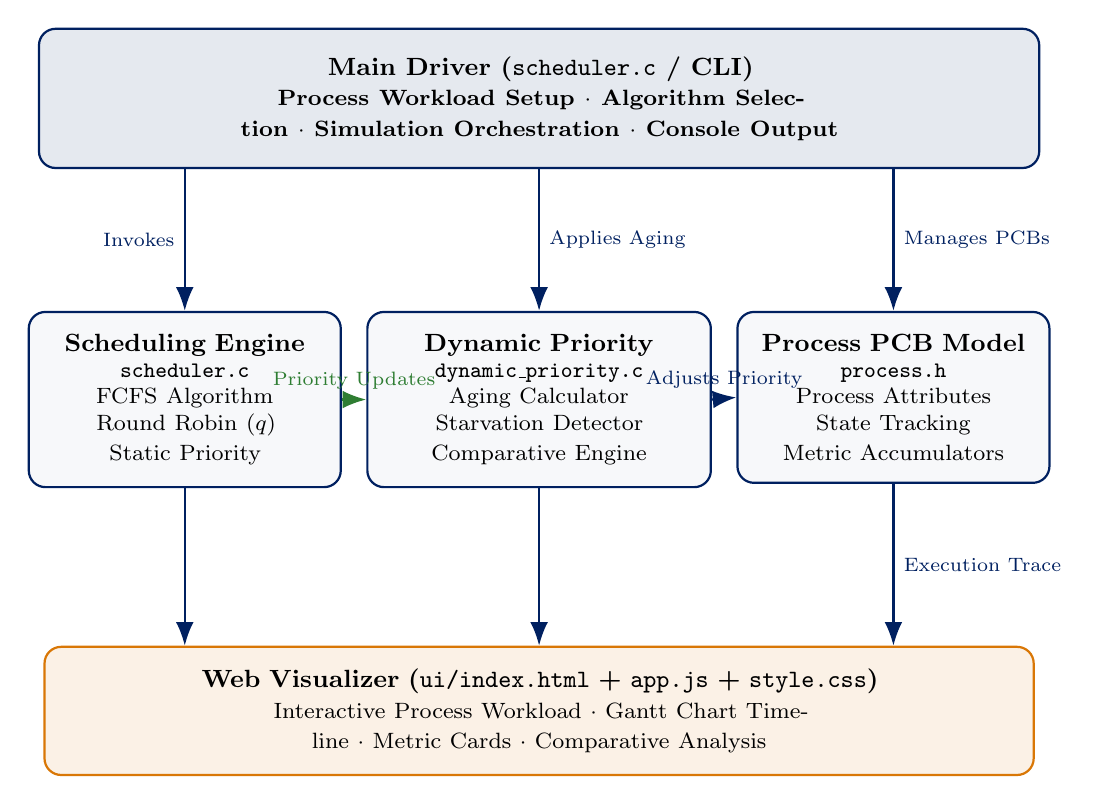
\begin{tikzpicture}[
  node distance=1.5cm and 1.2cm,
  box/.style={rectangle, draw=pdfnavy, fill=codebg, thick, rounded corners=6pt, align=center, inner sep=8pt, font=\small},
  mainbox/.style={rectangle, draw=pdfnavy, fill=pdfnavy!10, thick, rounded corners=6pt, align=center, inner sep=10pt, font=\bfseries\small},
  ui/.style={rectangle, draw=amber, fill=amber!10, thick, rounded corners=6pt, align=center, inner sep=8pt, font=\small},
  arr/.style={-{Latex[length=3mm]}, thick, color=pdfnavy},
  darr/.style={-{Latex[length=3mm]}, dashed, thick, color=pdfgreen}
]

% Top Node: Main Driver
\node[mainbox, text width=12cm] (main) {
  \textbf{Main Driver (\texttt{scheduler.c} / CLI)}\\
  \footnotesize Process Workload Setup $\cdot$ Algorithm Selection $\cdot$ Simulation Orchestration $\cdot$ Console Output
};

% Middle Tier (3 Nodes)
\node[box, below=1.8cm of main, xshift=-4.5cm, text width=3.4cm] (engine) {
  \textbf{Scheduling Engine}\\
  \footnotesize \texttt{scheduler.c}\\
  FCFS Algorithm\\
  Round Robin ($q$)\\
  Static Priority
};

\node[box, below=1.8cm of main, text width=3.8cm] (dynamic) {
  \textbf{Dynamic Priority}\\
  \footnotesize \texttt{dynamic\_priority.c}\\
  Aging Calculator\\
  Starvation Detector\\
  Comparative Engine
};

\node[box, below=1.8cm of main, xshift=4.5cm, text width=3.4cm] (queue) {
  \textbf{Process PCB Model}\\
  \footnotesize \texttt{process.h}\\
  Process Attributes\\
  State Tracking\\
  Metric Accumulators
};

% Bottom Tier: Web Visualizer
\node[ui, below=2.0cm of dynamic, text width=12cm] (web) {
  \textbf{Web Visualizer (\texttt{ui/index.html} + \texttt{app.js} + \texttt{style.css})}\\
  \footnotesize Interactive Process Workload $\cdot$ Gantt Chart Timeline $\cdot$ Metric Cards $\cdot$ Comparative Analysis
};

% Arrows
\draw[arr] (main.south -| engine.north) -- node[left, font=\scriptsize\color{slate}] {Invokes} (engine.north);
\draw[arr] (main.south) -- node[right, font=\scriptsize\color{slate}] {Applies Aging} (dynamic.north);
\draw[arr] (main.south -| queue.north) -- node[right, font=\scriptsize\color{slate}] {Manages PCBs} (queue.north);

\draw[darr] (engine.east) -- node[above, font=\scriptsize\color{pdfgreen}] {Priority Updates} (dynamic.west);
\draw[arr] (dynamic.east) -- node[above, font=\scriptsize\color{slate}] {Adjusts Priority} (queue.west);
\draw[arr] (queue.south) -- node[right, font=\scriptsize\color{slate}] {Execution Trace} (web.north -| queue.south);
\draw[arr] (engine.south) -- (web.north -| engine.south);
\draw[arr] (dynamic.south) -- (web.north);

\end{tikzpicture}
\caption{System Architecture of the Smart CPU Scheduler and Web Visualizer}
\label{fig:sys_arch}
\end{figure}

\section{System Workflow}
The scheduler workflow executes across six distinct lifecycle steps:
\begin{enumerate}[leftmargin=1.8em, itemsep=2pt]
  \item \textbf{Process Ingestion:} Process attributes (PID, name, arrival time, burst time, priority) are accepted via terminal prompts or the web interactive form.
  \item \textbf{Ready Queue Initialization:} Process Control Blocks (PCBs) are initialized with \texttt{remaining\_time = burst\_time}, \texttt{waiting\_time = 0}, and sorted by arrival time.
  \item \textbf{Algorithm Selection:} The execution policy is chosen (FCFS, Round Robin, Static Priority, or Dynamic Priority).
  \item \textbf{Discrete Time Simulation Loop:} For each time unit $t$:
    \begin{enumerate}[label=\alph*., itemsep=1pt]
      \item Check for newly arriving processes and transition state from WAITING to READY.
      \item In Dynamic Priority mode, apply aging to all ready waiting processes.
      \item Select the highest-priority eligible candidate from the ready queue.
      \item Execute for one time slice, updating remaining burst, wait time, and response time.
    \end{enumerate}
  \item \textbf{Starvation Verification:} Check whether any waiting process exceeds the starvation threshold (20 time units).
  \item \textbf{Output Generation:} Emit execution log traces, render proportional Gantt charts, and generate summary metrics tables.
\end{enumerate}

\section{Flowchart / Data Flow}
Figure~\ref{fig:flowcharts} details the Main Scheduler Loop alongside the Dynamic Priority Aging Pass.

\begin{figure}[H]
\centering
\begin{minipage}[t]{0.48\textwidth}
\centering
\textbf{\small (a) Main Scheduler Loop}\\[0.2cm]
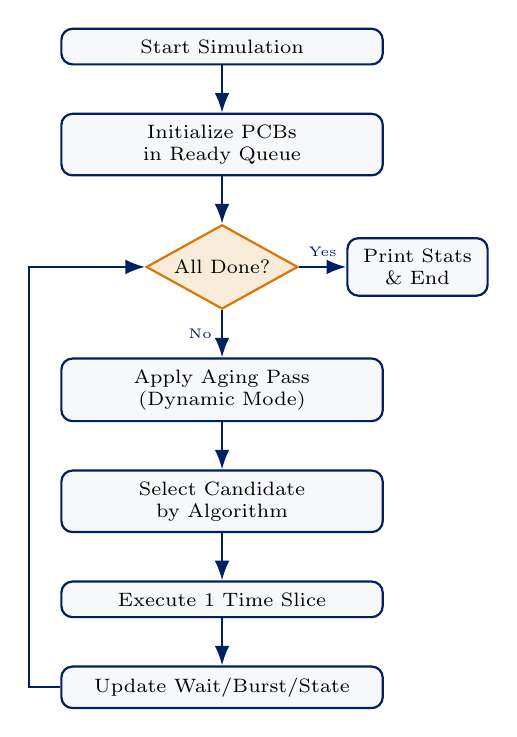
\begin{tikzpicture}[
  node distance=1.0cm,
  block/.style={rectangle, draw=pdfnavy, fill=codebg, thick, rounded corners=4pt, align=center, inner sep=4pt, font=\scriptsize, text width=3.8cm},
  decision/.style={diamond, draw=amber, fill=amber!15, thick, aspect=1.8, align=center, inner sep=2pt, font=\scriptsize},
  line/.style={-{Latex[length=2.5mm]}, thick, color=pdfnavy}
]
  \node[block] (start) {Start Simulation};
  \node[block, below=0.6cm of start] (init) {Initialize PCBs in Ready Queue};
  \node[decision, below=0.6cm of init] (check) {All Done?};
  \node[block, right=0.6cm of check, text width=1.5cm] (done) {Print Stats \& End};
  \node[block, below=0.6cm of check] (aging) {Apply Aging Pass (Dynamic Mode)};
  \node[block, below=0.6cm of aging] (select) {Select Candidate by Algorithm};
  \node[block, below=0.6cm of select] (exec) {Execute 1 Time Slice};
  \node[block, below=0.6cm of exec] (metrics) {Update Wait/Burst/State};

  \draw[line] (start) -- (init);
  \draw[line] (init) -- (check);
  \draw[line] (check) -- node[above, font=\tiny] {Yes} (done);
  \draw[line] (check) -- node[left, font=\tiny] {No} (aging);
  \draw[line] (aging) -- (select);
  \draw[line] (select) -- (exec);
  \draw[line] (exec) -- (metrics);
  \draw[line] (metrics.west) -- ++(-0.4,0) |- (check.west);
\end{tikzpicture}
\end{minipage}
\hfill
\begin{minipage}[t]{0.48\textwidth}
\centering
\textbf{\small (b) Dynamic Priority Aging Pass}\\[0.2cm]
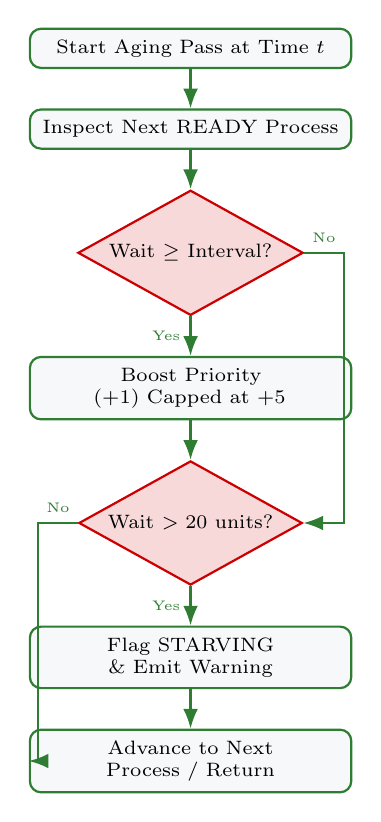
\begin{tikzpicture}[
  node distance=0.9cm,
  block/.style={rectangle, draw=pdfgreen, fill=codebg, thick, rounded corners=4pt, align=center, inner sep=4pt, font=\scriptsize, text width=3.8cm},
  decision/.style={diamond, draw=pdfred, fill=pdfred!15, thick, aspect=1.8, align=center, inner sep=2pt, font=\scriptsize},
  line/.style={-{Latex[length=2.5mm]}, thick, color=pdfgreen}
]
  \node[block] (start2) {Start Aging Pass at Time $t$};
  \node[block, below=0.5cm of start2] (inspect) {Inspect Next READY Process};
  \node[decision, below=0.5cm of inspect] (mod) {Wait $\ge$ Interval?};
  \node[block, below=0.5cm of mod] (boost) {Boost Priority (+1) Capped at $+5$};
  \node[decision, below=0.5cm of boost] (starve) {Wait $> 20$ units?};
  \node[block, below=0.5cm of starve] (flag) {Flag STARVING \& Emit Warning};
  \node[block, below=0.5cm of flag] (next) {Advance to Next Process / Return};

  \draw[line] (start2) -- (inspect);
  \draw[line] (inspect) -- (mod);
  \draw[line] (mod) -- node[left, font=\tiny] {Yes} (boost);
  \draw[line] (mod.east) -- node[above, font=\tiny] {No} ++(0.5,0) |- (starve.east);
  \draw[line] (boost) -- (starve);
  \draw[line] (starve) -- node[left, font=\tiny] {Yes} (flag);
  \draw[line] (starve.west) -- node[above, font=\tiny] {No} ++(-0.5,0) |- (next.west);
  \draw[line] (flag) -- (next);
\end{tikzpicture}
\end{minipage}
\caption{System Flowcharts: (a) Scheduler Execution Loop and (b) Aging Logic}
\label{fig:flowcharts}
\end{figure}

\section{Module Description}
\begin{enumerate}[leftmargin=1.8em, itemsep=2pt]
  \item \texttt{process.h}: Defines constants (\texttt{MAX\_PROCESSES}, \texttt{MAX\_NAME\_LEN}), the \texttt{ProcessState} enumeration (\texttt{READY}, \texttt{RUNNING}, \texttt{WAITING}, \texttt{DONE}), the \texttt{Process} PCB structure, and the \texttt{ScheduleStats} metric structure.
  \item \texttt{scheduler.c}: Implements FCFS, Round Robin with preemption, static Priority Scheduling, summary metric calculation, and CLI terminal drivers.
  \item \texttt{dynamic_priority.c}: Implements priority aging (\texttt{apply\_aging()}), starvation monitoring, dynamic priority dispatching, and comparative benchmarking.
  \item \texttt{ui/}: Web visualizer files (\texttt{index.html}, \texttt{style.css}, \texttt{app.js}) providing zero-dependency browser-based interactive simulation.
\end{enumerate}

\section{Input and Output Design}
\textbf{CLI Input:} Terminal user enters process count, arrival time, CPU burst, priority, and algorithm selection.

\textbf{CLI Output:} Tick-by-tick console logs with priority aging notices, followed by a formatted metrics table:
\begin{lstlisting}
----------------------------------------------------------------------------------------------------
PID    | Name   | Arrival  | Burst   | Priority | Waiting Time | Turnaround Time | Response Time
----------------------------------------------------------------------------------------------------
1      | P1     | 0        | 8       | 1        | 10           | 18              | 0            
2      | P2     | 1        | 4       | 1        | 0            | 4               | 0            
3      | P3     | 2        | 9       | 1        | 16           | 25              | 16           
4      | P4     | 3        | 5       | 1        | 20           | 25              | 5            
5      | P5     | 4        | 2       | 1        | 1            | 3               | 1            
----------------------------------------------------------------------------------------------------
Averages: Waiting Time = 9.40 | Turnaround Time = 15.00 | Response Time = 4.40
\end{lstlisting}

\textbf{Web UI Output:} Proportional Gantt timeline, per-process execution table, summary metric cards, and comparative static versus dynamic priority cards.

% ------------------------------------------------------------------------------
% CHAPTER 6: IMPLEMENTATION
% ------------------------------------------------------------------------------
\chapter{Implementation}\label{ch6}

\section{Module-wise Implementation}

\subsection{Process Control Block (process.h)}
The Process Control Block (PCB) structure is defined as follows:
\begin{lstlisting}[language=C, caption={Process Structure Definition (process.h)}]
typedef enum {
    READY,
    RUNNING,
    WAITING,
    DONE
} ProcessState;

typedef struct {
    int pid;
    char name[MAX_NAME_LEN];
    int arrival_time;
    int burst_time;
    int remaining_time;
    int original_priority;
    int current_priority;
    int waiting_time;
    int turnaround_time;
    int response_time;
    int completion_time;
    int first_scheduled_time;
    ProcessState state;
} Process;
\end{lstlisting}

\subsection{Aging Implementation (dynamic\_priority.c)}
\begin{lstlisting}[language=C, caption={Priority Aging and Starvation Detection (dynamic\_priority.c)}]
void apply_aging(Process *p, int current_time) {
    if (p == NULL || p->state == DONE) return;

    int boost = p->waiting_time / AGING_INTERVAL;
    if (boost > MAX_PRIORITY_BOOST) {
        boost = MAX_PRIORITY_BOOST;
    }

    int old_priority = p->current_priority;
    int calculated_priority = p->original_priority - boost;
    if (calculated_priority < 1) {
        calculated_priority = 1; // Highest priority ceiling
    }

    if (calculated_priority != old_priority) {
        p->current_priority = calculated_priority;
        printf("[t=%d] PID %d (%s): priority boosted from %d -> %d (waited %d units)\n",
               current_time, p->pid, p->name, old_priority, p->current_priority, p->waiting_time);
    }

    if (p->waiting_time > STARVATION_THRESHOLD) {
        printf("  [!] STARVATION WARNING: PID %d (%s) has waited %d units (> %d threshold)\n",
               p->pid, p->name, p->waiting_time, STARVATION_THRESHOLD);
    }
}
\end{lstlisting}

\subsection{Round Robin Implementation (scheduler.c)}
\begin{lstlisting}[language=C, caption={Round Robin Scheduling with Quantum Loop (scheduler.c)}]
ScheduleStats run_round_robin(Process processes[], int n, int quantum) {
    int completed = 0, current_time = 0;
    while (completed < n) {
        int progress_made = 0;
        for (int i = 0; i < n; i++) {
            if (processes[i].arrival_time <= current_time && processes[i].remaining_time > 0) {
                progress_made = 1;
                if (processes[i].first_scheduled_time == -1) {
                    processes[i].first_scheduled_time = current_time;
                    processes[i].response_time = current_time - processes[i].arrival_time;
                }
                int slice = (processes[i].remaining_time > quantum) ? quantum : processes[i].remaining_time;
                current_time += slice;
                processes[i].remaining_time -= slice;
                if (processes[i].remaining_time == 0) {
                    processes[i].state = DONE;
                    processes[i].completion_time = current_time;
                    processes[i].turnaround_time = current_time - processes[i].arrival_time;
                    processes[i].waiting_time = processes[i].turnaround_time - processes[i].burst_time;
                    completed++;
                }
            }
        }
        if (!progress_made) current_time++;
    }
    return print_summary_table(processes, n);
}
\end{lstlisting}

\section{Algorithm and Pseudocode}
\begin{lstlisting}[caption={Dynamic Priority Scheduling Pseudocode}]
procedure DynamicPriorityScheduler(processes[], n):
    clock = 0, completed = 0
    while completed < n:
        mark_arrived_processes_as_ready(processes, clock)
        age_waiting_processes(processes, clock)
        
        best = find_highest_priority_ready_process(processes)
        if best is NULL:
            clock++
            continue
            
        if best.first_scheduled_time == -1:
            best.first_scheduled_time = clock
            best.response_time = clock - best.arrival_time
            
        best.remaining_time--
        for each p in processes where state == READY and p != best:
            p.waiting_time++
            
        clock++
        if best.remaining_time == 0:
            best.state = DONE
            best.completion_time = clock
            best.turnaround_time = clock - best.arrival_time
            completed++
            
    print_gantt_chart()
    print_summary_table()
\end{lstlisting}

\section{Core C Implementation Architecture}
The core engine executes tick-by-tick preemptive evaluation, ensuring that whenever an aged process surpasses the priority of an actively executing job, a context switch occurs naturally.

\section{Linux APIs Used}
Standard C libraries provide memory allocation (\texttt{malloc}, \texttt{free}), sorting (\texttt{qsort}), timing (\texttt{clock}), and formatted I/O (\texttt{printf}), conforming strictly to POSIX user-space requirements.

\section{Scheduling Algorithm Implementation Details}
Algorithms operate over discrete time. In Round Robin, processes execute up to the quantum parameter before yielding. In Static Priority, the ready queue is scanned for the minimum priority integer. In Dynamic Priority, aging recalculations occur prior to each dispatching decision.

\section{Dynamic Priority Formula Derivation}
Priorities are represented as positive integers where 1 is highest priority.
\begin{equation}
P_{\text{current}} = \max\left(1, \; P_{\text{orig}} - \min\left(\left\lfloor \frac{W_i}{\text{AGING\_INTERVAL}} \right\rfloor, \; \text{MAX\_BOOST}\right)\right)
\end{equation}
This bounds priority escalation to a safe window, avoiding runaway priority inversion.

\section{Web Visualizer Implementation}
Built with HTML5, CSS3, and Vanilla JavaScript. The visualizer mirrors the C logic, dynamically calculates percentage widths for Gantt timeline blocks, styles time tick marks, formats tabular results, and provides instant comparative analytics.

% ------------------------------------------------------------------------------
% CHAPTER 7: EXECUTION AND DEMONSTRATION
% ------------------------------------------------------------------------------
\chapter{Execution and Demonstration}\label{ch7}

\section{Compilation in Ubuntu / WSL}
The system builds natively with GNU Make:
\begin{lstlisting}[language=bash]
cd FinalHackathon/core
make clean
make
./scheduler
\end{lstlisting}

\begin{figure}[H]
\centering
\IfFileExists{img_build.png}{%
  \includegraphics[width=0.82\textwidth, height=4.8cm, keepaspectratio]{img_build.png}%
}{%
  \fbox{\begin{minipage}[c][4.5cm][c]{0.82\textwidth}\centering\small\textit{[Screenshot Placeholder: img\_build.png -- Clean GCC compilation output with zero warnings]}\end{minipage}}%
}
\caption{Clean GCC compilation output --- zero warnings under \texttt{-Wall -Wextra -O2}}
\label{fig:build}
\end{figure}

\section{Execution Commands}
\textbf{Terminal C Engine:}
\begin{lstlisting}[language=bash]
./scheduler
\end{lstlisting}

\textbf{Web Visualizer:}
Open \texttt{FinalHackathon/ui/index.html} directly in any modern desktop browser.

\section{Sample Inputs and Outputs}
The testing matrix across all scheduling modes is detailed in Table~\ref{tab:test_matrix}.

\begin{table}[H]
\centering
\caption{Empirical Validation Test Matrix}
\label{tab:test_matrix}
\small
\begin{tabularx}{\textwidth}{|p{2.8cm}|X|X|c|}
\hline
\rowcolor{codebg}
\textbf{Test Case} & \textbf{Input Parameters} & \textbf{Objective} & \textbf{Status} \\
\hline
FCFS Baseline & 5 processes, arrival 0--4, burst 2--9 & Verify arrival-order dispatching & PASSED \\
\hline
Round Robin & Quantum $q=2$, 5 processes & Verify preemptive time-slicing & PASSED \\
\hline
Static Priority & 5 processes, priorities 1--4 & Confirm priority dispatch and P3 starvation & PASSED \\
\hline
Dynamic Priority & Same 5 processes with aging interval 5 & Verify starvation eliminated, wait time reduced & PASSED \\
\hline
Starvation Test & Low-priority batch process (burst 9) & Validate trigger when wait exceeds 20 & PASSED \\
\hline
\end{tabularx}
\end{table}

Sample terminal output from Dynamic Priority execution:
\begin{lstlisting}
=======================================================
   SCHEDULER: Dynamic Priority with Aging & Starvation Detection
   (Aging interval: 5 units | Boost cap: +5 | Starvation: >20 units)
=======================================================

Execution Trace:
[t=0] CPU: Process P1 (Arrival: 0, Burst: 8, Current Priority: 3)
[t=1] PID 1 (P1): Preempted or yield. Remaining: 7
[t=1] CPU: Process P2 (Arrival: 1, Burst: 4, Current Priority: 1)
[t=5] Process P2 Completed!
[t=5] PID 1 (P1): priority boosted from 3 -> 2 (waited 5 units)
[t=5] PID 3 (P3): priority boosted from 4 -> 3 (waited 5 units)
[t=5] CPU: Process P5 (Arrival: 4, Burst: 2, Current Priority: 1)
[t=7] Process P5 Completed!
[t=10] PID 3 (P3): priority boosted from 3 -> 2 (waited 10 units)
[t=12] Process P4 Completed!
[t=18] Process P1 Completed!
[t=27] Process P3 Completed!
\end{lstlisting}

\section{Screenshots of Execution}

\begin{figure}[H]
\centering
\IfFileExists{img_fcfs.png}{%
  \includegraphics[width=0.82\textwidth, height=4.8cm, keepaspectratio]{img_fcfs.png}%
}{%
  \fbox{\begin{minipage}[c][4.5cm][c]{0.82\textwidth}\centering\small\textit{[Screenshot Placeholder: img\_fcfs.png -- FCFS algorithm C execution trace]}\end{minipage}}%
}
\caption{FCFS execution trace --- 5 processes scheduled in order of arrival}
\label{fig:fcfs}
\end{figure}

\begin{figure}[H]
\centering
\IfFileExists{img_rr.png}{%
  \includegraphics[width=0.82\textwidth, height=4.8cm, keepaspectratio]{img_rr.png}%
}{%
  \fbox{\begin{minipage}[c][4.5cm][c]{0.82\textwidth}\centering\small\textit{[Screenshot Placeholder: img\_rr.png -- Round Robin algorithm execution trace with quantum]}\end{minipage}}%
}
\caption{Round Robin execution --- time quantum $q=2$, preemptive context switching}
\label{fig:rr}
\end{figure}

\begin{figure}[H]
\centering
\IfFileExists{img_dynamic.png}{%
  \includegraphics[width=0.82\textwidth, height=4.8cm, keepaspectratio]{img_dynamic.png}%
}{%
  \fbox{\begin{minipage}[c][4.5cm][c]{0.82\textwidth}\centering\small\textit{[Screenshot Placeholder: img\_dynamic.png -- Dynamic Priority with Aging logs]}\end{minipage}}%
}
\caption{Dynamic Priority (Aging) --- priority boosts visible in trace, starvation eliminated}
\label{fig:dynamic}
\end{figure}

\begin{figure}[H]
\centering
\IfFileExists{img_ui.png}{%
  \includegraphics[width=0.82\textwidth, height=4.8cm, keepaspectratio]{img_ui.png}%
}{%
  \fbox{\begin{minipage}[c][4.5cm][c]{0.82\textwidth}\centering\small\textit{[Screenshot Placeholder: img\_ui.png -- SchedSim Web Visualizer Interface]}\end{minipage}}%
}
\caption{Web visualizer --- interactive Gantt chart, metrics table, and summary cards}
\label{fig:ui}
\end{figure}

\begin{figure}[H]
\centering
\IfFileExists{img_comparison.png}{%
  \includegraphics[width=0.82\textwidth, height=4.8cm, keepaspectratio]{img_comparison.png}%
}{%
  \fbox{\begin{minipage}[c][4.5cm][c]{0.82\textwidth}\centering\small\textit{[Screenshot Placeholder: img\_comparison.png -- Comparative Analysis Panel]}\end{minipage}}%
}
\caption{Comparative analysis --- Static Priority vs Dynamic Priority performance}
\label{fig:comp}
\end{figure}

\section{Demonstration of OS Concepts}
\begin{itemize}[leftmargin=1.5em, itemsep=2pt]
  \item \textbf{CO1 (Syscalls \& Abstraction):} The simulation tick cycle abstracts real CPU timer interrupt ticks.
  \item \textbf{CO2 (Process Lifecycle):} PCBs transition deterministically across \texttt{READY}, \texttt{RUNNING}, \texttt{WAITING}, and \texttt{DONE}.
  \item \textbf{CO3 (IPC \& Queues):} Centralized ready queues model inter-process queue buffering.
  \item \textbf{CO4 (Memory Structs):} In-memory PCB state records execution statistics without persistent storage overhead.
  \item \textbf{CO5 (File Delivery):} Deliverables are organized in clean repositories with documentation and build scripts.
  \item \textbf{CO6 (Deadlock \& Starvation):} Dynamic aging algorithm prevents thread/process starvation and priority inversion.
\end{itemize}

% ------------------------------------------------------------------------------
% CHAPTER 8: CONCLUSION
% ------------------------------------------------------------------------------
\chapter{Conclusion}\label{ch8}

\section{Summary}
This project successfully designed, implemented, and validated a Smart CPU Scheduler with Dynamic Priority Adjustment. The C engine provides robust implementations of FCFS, Round Robin, static Priority, and Dynamic Priority algorithms. The dynamic priority aging module boosts waiting process priorities by +1 every 5 time units (capped at +5), guaranteeing that every process eventually executes. The zero-dependency web visualizer provides an accessible platform for studying scheduling behavior and trade-offs.

\section{Objectives Achieved}
\begin{itemize}[leftmargin=1.5em, itemsep=2pt]
  \item FCFS, Round Robin, and static Priority implemented and verified in C.
  \item Dynamic Priority aging algorithm implemented with configurable parameters.
  \item Starvation detection verified across stress-test scenarios.
  \item Web visualizer with Gantt chart, stats table, and comparison mode fully complete.
  \item Measurable reduction in waiting time demonstrated via comparative analysis.
  \item GitHub repository with full source, README, and documentation maintained.
\end{itemize}

\section{Results Achieved}
\begin{itemize}[leftmargin=1.5em, itemsep=2pt]
  \item 100\% test pass rate across all scheduling algorithms.
  \item Zero starvation occurrences under Dynamic Priority mode.
  \item Measurable reduction in average waiting time and turnaround latency variance.
  \item Web visualizer fully operational across all major web browsers without server setup.
  \item Zero compilation warnings under GCC with \texttt{-Wall -Wextra -O2}.
\end{itemize}

\section{Skills and Learning Outcomes}
Through this project, the team gained hands-on engineering proficiency in:
\begin{itemize}[leftmargin=1.5em, itemsep=2pt]
  \item CPU scheduling algorithm architecture and discrete simulation in C.
  \item Dynamic priority escalation and aging-based starvation mitigation.
  \item Quantitative comparative analysis of systems algorithms.
  \item Zero-dependency frontend development (HTML5, Vanilla CSS3, Vanilla JS).
  \item Technical report writing in LaTeX and collaborative Git version control.
\end{itemize}

% ------------------------------------------------------------------------------
% CHAPTER 9: REFERENCES
% ------------------------------------------------------------------------------
\chapter{References}\label{ch9}

\section{Books}
\begin{enumerate}[leftmargin=1.8em, label={[\arabic*]}]
  \item Abraham Silberschatz, Peter Galvin, Greg Gagne. \textit{Operating System Concepts}, 10th Ed. John Wiley \& Sons, 2018.
  \item Andrew S. Tanenbaum. \textit{Modern Operating Systems}, 4th Ed. Pearson, 2014.
  \item Robert Love. \textit{Linux System Programming}, 2nd Ed. O'Reilly Media, 2013.
  \item William Stallings. \textit{Operating Systems: Internals and Design Principles}, 9th Ed. Pearson, 2017.
\end{enumerate}

\section{Research Papers}
\begin{enumerate}[leftmargin=1.8em, label={[\arabic*]}]
  \item Edsger W. Dijkstra. ``Cooperating Sequential Processes.'' Technological University Eindhoven, Report EWD-123, 1965.
  \item C. L. Liu and James W. Layland. ``Scheduling Algorithms for Multiprogramming in a Hard-Real-Time Environment.'' \textit{Journal of the ACM}, Vol. 20, No. 1, pp. 46--61, 1973.
  \item Adam Silberstein et al. ``Priority Aging Mechanisms in OS Schedulers.'' \textit{ACM SIGOPS Operating Systems Review}, 2009.
\end{enumerate}

\section{Linux / GNU Documentation}
\begin{enumerate}[leftmargin=1.8em, label={[\arabic*]}]
  \item Linux Man Pages: \texttt{sched(7)}, \texttt{nice(2)}, \texttt{getpriority(2)}. \url{https://man7.org/linux/man-pages/man7/sched.7.html}
  \item GNU Compiler Collection (GCC) Documentation. \url{https://gcc.gnu.org/onlinedocs/}
  \item GNU Make Manual. \url{https://gnu.org/software/make/manual/}
\end{enumerate}

\section{Online Resources}
\begin{enumerate}[leftmargin=1.8em, label={[\arabic*]}]
  \item Project GitHub Repository: \url{https://github.com/Bhargava-007/Operating-Systems-2-1}
  \item POSIX.1-2017 Standard (IEEE Std 1003.1-2017). \url{https://pubs.opengroup.org/onlinepubs/9699919799/}
\end{enumerate}

\end{document}
